
\documentclass[a4paper,11pt,norsk]{article}
\usepackage[utf8]{inputenc}
%\usepackage[utf8]{inputenc}
\usepackage{a4wide}
\usepackage{lmodern}
\usepackage[T1]{fontenc}
\usepackage{babel}
\setlength{\parindent}{0pt} 
\setlength{\parskip}{2ex}
\usepackage{fixltx2e}
\usepackage{amsmath}
\usepackage[pdftex, pdfborderstyle={/S/U/W 0}]{hyperref}
\usepackage{graphicx}
\usepackage[font=small,labelfont=bf]{caption}
\usepackage{}
\usepackage{tabularx}
\usepackage{multirow}
\usepackage[american]{circuitikz}
\usetikzlibrary{arrows,shapes,positioning,calc}
\usetikzlibrary{decorations.markings}

\begin{document}

%Headingdel:---------------------------------------------
\begin{minipage}[c]{0.15\textwidth}

\includegraphics[width=2.0cm]{img/elsys_pos_staaende_ntnu}  
\end{minipage}
\begin{minipage}[c]{0.85\textwidth}

\renewcommand{\arraystretch}{1.7}
\large 
\begin{tabularx}{\textwidth}{|X|X|}
\hline
\multicolumn{2}{|l|}{} \\
\multicolumn{2}{|l|}{\huge \textbf{Rapport Arbeider 2}} \\
\multicolumn{2}{|l|}{}  \\
\hline
\multicolumn{2}{|l|}{Tittel: 
%Skriv inn tittel her:------------------------------------------
Sinusgenerator med valgfri amplitude og offset
} \\
\hline
\multicolumn{2}{|l|}{Forfattere: 
%Skriv inn forfattere her:--------------------------------------
Sindre Danielsen
} \\
\hline
%Skriv inn versjon og dato her her:-----------------------------
Versjon: 4.0 & Dato: 06.06.21
\\
\hline 
\end{tabularx}
\end{minipage}
\normalsize

%Automatisk generert innholdsfortegnelse:------------------

\setlength{\parskip}{0ex}
\renewcommand{\baselinestretch}{0.1}\normalsize
\tableofcontents
\renewcommand{\baselinestretch}{1.00}\normalsize
\setlength{\parskip}{2ex}
\rule{\textwidth}{1pt}

%Selve rapporten:------------------------------------------
\newpage
\section{Introduksjon}
\label{sec:innledning}
Det er ikke alltid man har tilgang på en sinusgenerator, så vi skal nå se på hvordan vi kan utvikle det selv. I tillegg kan det også være nyttig at signalet kan variere rundt en hvilken som helst konstant spenning (offset). Figur~\ref{fig:generell_singenerator} viser et slikt system.
% Lag en circuittikz her
\begin{figure}[htbp]
    \centering
    \begin{circuitikz} [american voltages, european resistors, baseline=(current bounding box.center)]
        \ctikzset { label/align = straight }
        \draw
        % Bottom-right side
        % V trekantsignal
        (4, 2) to[short, -o] (5,2)
        to[short] (6,2)
        % V_
        (2,0) to[short] (2,-1)
        to[short,l=$V_-$,-o] (2,-1)
        % V+
        (2,4) to[short] (2,5)
        to[short, l=$V_+$,-o] (2,5)
        ;
        \node at (5,2.5) (PSU_l){$v(t)$};
        
        
        % Nivåregulator
        \node[draw,minimum width=4cm,minimum height=4cm,anchor=south west] at (0,0){\textbf{Sinusgenerator}};

        
    \end{circuitikz}
    \caption{Sinusgenerator med offset.}
  \label{fig:generell_singenerator}
\end{figure} \\
Systemet skal ta inn to konstante spenningskilder $V_+$ og $V_-$, som er like store og motsatt retning. Det vi skal få ut er et et sinussignal $v(t)$ med en amplitude $A$ og en offset $V_0$, som gir oss et signal på formen:
\begin{equation}
    v(t) = A \cos{(2\pi f t)} + V_0 \quad , \quad \textit{der $f$ betegner frekvensen på signalet.}
\end{equation}\label{eq:v_2}
\\\\
For at systemet skal yte godt nok, så kreves det en frekvensnøyaktighet på $10\: 000$ppm, samt en Signal-Distorsjons-Ratio (SDR) større enn 20dB. Dette viser seg å være det som er minimums anbefalte ratioen.
\\\\
\textbf{Merk at:} Systemet nullstiller ikke faseforskyvninger på utgangssignalet $v(t)$.


\newpage
\section{Problembeskrivelse, konsept og design}
En metode for å utvikle en sinusgenerator på er gjennom flere delsystemer, som er vist i figur~\ref{fig:sin_delsystemer}. \\
\begin{figure}[htbp]
    \centering
    \begin{circuitikz} [american voltages, european resistors, baseline=(current bounding box.center)]
        \ctikzset { label/align = straight }
        \draw
        %Komperator
        % V_
        (6.4,-0.90) to[short] (6.4,-1.90)
        to[short,l=$V_-$,-o] (6.4,-1.90)
        % V+
        (6.4,2.9) to[short] (6.4,3.9)
        to[short, l=$V_+$,-o] (6.4,3.9);
        % Between systems

        %Top between systems
        \draw[-latex] (7.5,1) -- (8.5,1);
        
        % Integrator
        % Bottom-right side
        \draw[-latex] (11.75,1) -- (12.75,1);
        
        % To offset
        \draw[-latex] (15.75,1) -- (16.75,1);
        \draw node[label={$v(t)$}] at (19.25,1);
        \draw[-latex] (18.25,1) -- (19.25,1);
        % Nivåregulator
        \node[draw,minimum width=3cm,minimum height=3.8cm,anchor=south west] at (4.5,-0.90){\textbf{\begin{tabular}{c}
             &  Firkant\\
             & Generator
        \end{tabular}}};
        \node[draw,minimum width=3cm,minimum height=3.8cm,anchor=south west] at (8.5,-0.90){\textbf{{\textbf{\begin{tabular}{c}
             &  3. Ordens\\
             & Lavpass filter \\
             (Aktiv)
        \end{tabular}}}}};
        \node[draw,minimum width=3cm,minimum height=3.8cm,anchor=south west] at (12.75,-0.90){\textbf{{\textbf{\begin{tabular}{c}
             &  Spennings-\\
             & demper
        \end{tabular}}}}};
        \node[draw,minimum width=1.5cm,minimum height=3.8cm,anchor=south west] at (16.75,-0.90){\textbf{Offset}};
        

        
    \end{circuitikz}
    \caption{Sinusgeneratorens delsystemer.}
  \label{fig:sin_delsystemer}
\end{figure} \\
Det krever først at vi omformer to likespenninger ($V_+$ og $V_-$) om til vekselspenning, som lar enkelt lar seg gjøre ved bruk av en firkantgenerator. Firkantsignalet som utvikles må filtreres minst tre ganger ved hjelp av lavpass filter, for å få et tilnærmet sinussignal. Dette kan gjøres ved enten passivt eller aktivt lavpass filter.
Der et passivt lavpass filter består av en motstand og en kondensator i paralell, samt en op-amp forsterker etterpå.
Et aktivt lavpass filter har motstand og kondensator i parallell, som negativ feedback på en op-amp. Vi bruker her et aktivt lavpass filter for å utvikle et sinussignal, slik vist i  figur~\ref{fig:sin_filter}.
For at signalet nå skal være av den amplituden ønsket, så brukes en spenningsdemper. Siste ledd i systemet er å legge til en konstant spenningskilde til sinussignalet, slik at vi får en offset.
\\\\
\textbf{Merk at:} For at systemet skal fungere optimalt, så brukes buffere etter firkantsignalet og etter spenningsdemperen. Op-ampene etter hver filtreringene opererer som forsterkere av signalet.

Dette blir inkludert i hvert kretsdesign i de følgende delseksjonene i denne seksjonen. \\
Det er to årsaker for å bruke buffere: \\
1) Isolasjon av spenningen og strømmen i deler av kretsen, der det er ønskelig, slik at ulike deler av kretsen ikke påvirker hverandre. \\
2) Buffere med forsterkning oppfører seg som i 1) og vil også øke styrken på signalet, dersom signalet skulle miste styrke (amplitude) i kretsen.\\\\

\label{sec:prinsipielllosning}
Siden sinusgeneratoren består av flere delsystemer, så tar vi for oss kretsene til delsystemene hver for seg. Legg merke til at bufferene ikke er merket med spenningsforsyningene $V_-$ og $V_+$ i kretsskjemaene. Det er underforstått at de gjelder for enhver op-amp brukt i systemet.
\newpage
\subsection{Firkantgenerator}
En firkantgenerator kan vi utvikle ved hjelp av en komparator og en buffer slik vist i figur~\ref{fig:firkantgenerator}. \\
\begin{figure}[htbp]
    \centering
    \begin{circuitikz}
        % Circuit to comparator
        \draw (0.5, 0)
        to[C, l_=$C_1$] (-1,0)
        node[ground]{} (-1, -2)
        
        ;
        \draw(0, 0)
        to[short] (1,0)
        to[short] (1.5,0)
        (2.70,-0.490) node[op amp, label=$1$] (opamp) {}
        (opamp.up) ++ (0,.5) -- (opamp.up)
        (opamp.down) ++ (0,-.5) -- (opamp.down)
        node[label=$V_+$] at (2.70, .3)
        node[label=$V_-$] at (2.70, -2.3)
        ;
        
        % Grounding op-amp
        \draw (1.505,-0.97) to[short] (1.505, -3.50)
        to[european resistor, l=$R_1$] (1.505,-4.75)
        ;
        \draw (1.505,-4.75) to (1.505,-4.80) node[ground]{}; 
        ;
        \draw (1.505, -3.00)
        to[european resistor, l=$R_2$] (3.90,-3.00)
        to[short] (3.90,-.5)
        to[short,-o] (4.95, -.5)
        node[label=$v_1$] at (4.95,-.5)
        ;
        % All except op-amp
        \draw (1,0)
        % R2
        to[short,o-] (1,2)
        to[european resistor, l=$R_3$] (3.90,2)
        to[short,-o] (3.90,-.5);
        %node[right]{$v_1$};
        
        % Buffer
        \draw (7, -1) node[op amp,yscale=-1, label=$2$] (opamp) {}
        (opamp.+) to[short] (5, -.5)
        (opamp.-) |- (6, 0.25-2.5) to[short] (8, 0.25-2.5) -| (opamp.out)
        (opamp.out) to[short,o-] (8.2, -0.5)
        to[short,-o] (9.7, -0.5)
        node[label=$v_2$]
        to[short] (10.7, -0.5)
        ;
        \node[draw,dashed,minimum width=6.5cm,minimum height=9cm,anchor=south west, label={Komparator}]at (-2,-6) ;
        \node[draw,dashed,minimum width=3cm,minimum height=3cm,anchor=south west, label={Buffer}]at (5.5,-2.6) ;

        \end{circuitikz}
    \caption{Firkantgenerator \cite{r2} med buffer mellom $v_1$ og $v_2$.}
    \label{fig:firkantgenerator}
\end{figure}
\\
Komparatoren funker slik at den vil hele tiden måle differansen mellom den negative polen $V_2$ og positive polen $V_1$ på op-amp 1, som vi kaller $V_{id} = V_1 - V_2$. \\
Ved tiden $t=0$, så vil kondensatoren $C_1$ være tom og derfor vil $V_2 = 0$V. \\
Siden det forekommer forskjeller på $V_+$ og $V_-$, så vil vi få en $v_1 = V_+$ eler $v_1 = V_-$, avhengig av hvilken av $V_+$ og $V_-$ som er størst. \\
Anta at vi får $v_1 = V_+$, som gir en $+V_1$. 
For dette tilfellet vil $C_1$ fylle seg opp til den er større enn $+V_1$. Tilstanden endres slik at $V_{id} < 0$V, som gir $v_1 = V_-$.
$C_1$ tømmes ved at $R_3$ trekker på den, og $V_{id} < 0$V til $C_1$ har en spenning mindre enn $-V_1$, hvor tilstanden igjen vil endres til å $v_1 = V_+$, og prossessen gjentaes hele tiden.
Hvor fort dette går avhenger av hvor fort kondensatoren fylles og ''slew rate'' på op-amp 1 (finner i et datablad for modellen brukt).
\\\\
Mellom $v_1$ og $v_2$ setter vi inn en buffer (op-amp 2), slik at kretser tilkoblet firkantgeneratoren ikke vil forstyrre firkantsignalet som genereres.
\newpage
Firkantsignalet har en frekvens:
\begin{equation}
    f_0 = \frac{1}{2\pi R_3 C_1 \ln \left( \frac{2R_1 + R_2}{R_2} \right)}.
\end{equation}\label{eq:freq_advanced}
\\
Dersom vi velger $R_2 = 1.16 R_1$, så får vi en forenklet likning:
\begin{equation}
    f_0 = \frac{1}{2R_3 C_1}
    \label{eq:freq_simple}
\end{equation}
\\
$R_1$, $R_2$ og $R_3$ er motstandsverdiene i kretsen.
\\
\newpage
\subsection{3. Ordens filtrering}\label{sec:filters}
Dersom vi har et firkantsignal, så kan 3. Ordens filtrering brukes for å utvikle godt tilnærmet sinussignal. Det vil si å seriekoble tre lavpass filtre (RC-kretser) ved bruk av en krets kalt ''integrator''. Kretsdesignet til et lavpass filter er vist i figur~\ref{fig:sin_filter}.

\begin{figure}[htbp]
    \centering
    \begin{circuitikz} [american voltages, european resistors, european vresistors, baseline=(current bounding box.center)]
        \ctikzset { label/align = straight }
        
        \draw (1,0)
        node[label=$v_2$]
        to[R=$R_{i}$,o-] (4,0)
        to[short] (5,0)
        to[short] (5,4)
        to[C=$C_f$] (8.2, 4)
        to[short] (8.2,-.5);
        \draw (5,2) to[R=$R_f$] (8.2,2)
        ;
        % Buffer
        \draw (7, -0.5) node[op amp,yscale=1, label=$3$] (opamp) {}
        (opamp.-) to[short] (4, 0)
        (opamp.out) to[short] (8.2, -0.5)
        to[short,-o] (9.7, -0.5)
        node[label=$v_3$]
        ;
        \draw (opamp.+)
        node[ground] at (opamp.+);
        
        \node[draw,dashed,minimum width=7.5cm,minimum height=7.5cm,anchor=south west, label={Integrator}]at (1.5,-2.4) ;
        
    \end{circuitikz}
    \caption{Aktivt lavpass filter \cite{r3}.}
    \label{fig:sin_filter}
\end{figure} \\
Et 3. ordens lavpass filter består av å koble tre integratorer sammen i serie, for å få et signal som har en god tilnærming til et sinussignal, dersom inngangssignalet er firkantformet.
Vi kan bestemme verdiene på motstandene $R_i$ og $R_f$, samt kondensatoren $C_f$ gjennom formelen for en RC-krets:
\begin{equation}
    f_0 = \frac{1}{2\pi R_f C_f}.
    \label{eq:lavpass_filter}
\end{equation}
\\
Utgangssignalet $v_3$ får en forsterkning på:
\begin{equation}
    A = - \frac{R_f}{R_i}
\end{equation} \\
\\
Vi ønsker å holde signalets styrke lik gjennom hele kretsen, og dersom vi velger $A = 1$, så kan vi beholde samme $R_i$, $R_f$ og $C_f$ for hver filtrering.
\newpage

\subsection{Spenningsdemper}
Sinussignalet vi skal utvikle skal være av en viss styrke, som vi kan oppnå ved å bruke en spenningsdemper slik vist i figur~\ref{fig:spenningsdemper}.
\begin{figure}[htbp]
    \centering
    \begin{circuitikz} [american voltages, european resistors, european vresistors, baseline=(current bounding box.center)]
        \ctikzset { label/align = straight }
        \draw (0,0)
        node[label=$v_3$]
        to[short, o-] (2.5,0)
        to[R=$R_{D1}$] (2.5, -2)
        to[R=$R_{D2}$] (2.5, -6)
        (2.75,-7) node[below] {Spenningsdemper}
        ;
        \draw (2.5,-3) to[short, -o](6, -3)
        node[label=$v_4$]
        ;
        \draw node[ground] at (2.5,-6)
        ;
        \node[draw,dashed,minimum width=3.5cm,minimum height=8cm,anchor=south west] at (1,-7);
        
        
    \end{circuitikz}
    \caption{Spenningsdemper.}
    \label{fig:spenningsdemper}
\end{figure} \\
Utgangssignalet $v_4$ ønsker vi skal ha en forsterkning $A\in<0, 1>$, slik at $v_4$ er svekket:
\begin{equation}
    v_4 = A v_3.
    \label{eq:gain}
\end{equation} \\
Forsterkningen $A$ er bestemt av størrelseforholdet mellom motstanden $R_{D1}$ og $R_{D2}$:
\begin{equation}
    v_4 = v_3 \frac{R_{D2}}{R_{D1} + R_{D_2}}.
    \label{eq:spenningsdemper}
\end{equation}
\\
Det lurt å legge til en buffer etter $v_4$, som ikke er tilføyet dette kretsskjemaet.
\newpage
\subsection{Offset-system}
For å få en offset på sinussignalet, så brukes en summeringsforsterker, slik vist i figur~\ref{fig:summing_amplifier}.
\begin{figure}[htbp]
    \centering
    \begin{circuitikz}
        % Buffer
        \draw (7, -1) node[op amp,yscale=-1, label=$5$] (opamp) {}
        (opamp.-) |- (7, -3.5)
        to[european resistor,l=$R_A$] (9.7,-3.5)
        to[short] (9.7,-1)
        (opamp.+) |- (5, -.5)
        (opamp.out) to[short] (9.2, -1)
        to[short] (9.7, -1)
        to[short,-o] (10.7, -1)
        node[label=$v_5$]
        ;
        \draw (5.8, -3.5) to[european resistor, l=$R_B$] (5.8, -5.5)
        node[ground] at (5.8, -5.5);
        \draw (5,-.5) to[short]  (5,0)
        to[european resistor, l=$R_{4}$,-o] (5-3, 0)
        node[label=$v_4$]
        ;
         \draw (0.8, -1.5) node[op amp,yscale=-1, label=$4$] (opamp) {}
        (opamp.+) to[short] (-2, -1)
        to[european resistor, l=$R_{r}$] (-2, -3)
        to[V=$V_i$] (-2, -5)
        (opamp.-) to[short] (-.38,-3)
        to[short] (2,-3)
        to[short] (2,-1.5)
        ;
        \draw (-2, -1) to[european resistor, l=$R_{os}$] (-2, 2)
        node[ground, yscale=-1] at (-2, 1.5)
        ;
        \draw (5,-.5) to[short] (5,-1.5)
        to[european resistor, l=$R_{4}$,-o] (5-3, -1.5)
        node[above, label=$V_{0}$] at (5-3, -1.5)
        ;
        \draw node[ground] at (-2,-5); 
        \node[draw,dashed,minimum width=2.2cm,minimum height=9cm,anchor=south west, label={Offset spenningen}]at (-3,-6.5) ;
        \node[draw,dashed,minimum width=7.5cm,minimum height=7.5cm,anchor=south west, label={Ikke Inverterende Summeringsforsterker}]at (2.5,-6.5) ;
        \end{circuitikz}
    \caption{Summmeringsforsterker \cite{r1}: Addisjon av et AC og et DC signal, som gir en DC offset.}
    \label{fig:summing_amplifier}
\end{figure}
\\
Kresten tar inn et sinussignal $v_5$ og en spenningskilde $V_i$. Spenningskildene er ofte 5V, 12V eller liknende, så dersom vi ønsker en offset mindre enn dette, så legger vi til spenningsdeler over motstanden $R_r$ og $R_{os}$, som svekker styrken på signalet slik at vi får en ønsket likespenning $V_{0}$. \\
For å sørge for at offset-signalet $V_{0}$ skal være av den styrken ønsket, uansett hva motstanden $R_4$ er, så brukes en buffer mellom ''offset spenningen'' og den ''ikke inverterende summeringsforsterkeren''.
$V_{0}$ er gitt ved spenningsdeling:
\begin{equation}
    V_{0} = V_i \frac{R_{os}}{R_{os} + R_r}.
    \label{eq:spenningsdeling_offset}
\end{equation}
\\
Inngangsignalene på den ikke inverterende forsterkeren er $v_4$ og $V_{0}$. Disse står i paralell, slik at vi har et inngangsignal $V_{in}$ på den positive polen på op-amp 5:
\begin{equation}
    V_{in} = \frac{v_4 + V_{0}}{2}
    \label{eq:V_in}
\end{equation}\\
Den ikke inverterende forsterkeren skaper en forsterkning på utgangssignalet $v_5$:
\begin{equation}
    A = \frac{v_5}{V_{in}} = 1 + \frac{R_A}{R_B}
    \label{eq:gain}
\end{equation}
\\
Dersom $R_A = R_B$, så kan vi bruke likning~\ref{eq:V_in} til å forenkle likning~\ref{eq:gain}:
\begin{equation}
    v_5 = v_4 + V_{0}
\end{equation}
\\
For å få en amplitude på $v_5$ lik $v_4$, så settes $R_A = R_B = R_4$.
\\\\
Merk at: En inverterende op-amp gir mer stabilitet på signalet, men for å unngå bruke en ekstra inverterer på slutten av systemet, så velges en ikke inverterende summeringsforsterker.
\newpage
\section{Realisering og verifikasjon}
\label{sec:realisering}
De generelle verdiene for sinusgeneratoren er gitt ved tabell~\ref{table:slutt_resultat}. \\
\begin{table}[htbp]
\centering
\begin{tabular}{ |c|c|c|c| } 
\hline
\textbf{Navn} & \textbf{Verdi} & \textbf{Beskrivelse} \\
\hline
$f_0$ & $3.5$kHz  & Valgfri verdi\\
\hline
$A$ & $0.2$V & Valgfri verdi\\
\hline
$V_0$ & $0.7$V & Valgfri verdi \\ 
\hline
$V_+ / V_-$ & ~ \pm5V & Vanlig for småelektronikk. \\
\hline
Op-amp & LF353P & \\ 
\hline
\end{tabular}
\caption{Generelle verdier for sinusgeneratoren.}
\label{table:slutt_resultat}
\end{table}
\subsection{Firkantgeneratoren}
Verdiene brukt i firkantgeneratoren er vist ved tabell~\ref{table:variabler}.
\begin{table}[htbp]
\centering
\begin{tabular}{ |c|c|c|c| } 
\hline
\textbf{Navn} & \textbf{Verdi} & \textbf{Beskrivelse} \\
\hline
$R_1$ & $1232\Omega$ & $R_2 / 1.16$ \\ 
\hline
$R_2$ & $1429\Omega$ & Lik $R_3$ \\
\hline
$R_3$ & $1429\Omega$ & Likning~\ref{eq:freq_simple} \\
\hline
$C_1$ & $100$nF & Valgri verdi (likning~\ref{eq:freq_simple}) \\
\hline
\end{tabular}
\caption{Verdier brukt i firkantgeneratoren.}
\label{table:variabler}
\end{table}
\\
Firkantgeneratoren lager et signal før bufferen er tilkoblet vist ved figur~\ref{fig:square_before_buffer}.
Etter bufferen er tilkoblet ser vi et bedre firkantsignal, vist ved figur~\ref{fig:square_after_buffer}.
Begge har et utgangssignal med lavere amplitude enn på inngangssignalet. Dette kan blant annet skyldes kvaliteten på op-ampene som blir brukt, samt at systemet bruker kabler av unødvendig stor lengde. Ved måling får vi $f_0 \in <3.39$kHz$, 3.41$kHz$>$, som ikke er innenfor ønsket frekvensnøyaktighet nevnt i seksjon~\ref{sec:innledning}. Dette kommer av at motstandene brukt i utvikling av kretsen har avvik på$ <0\Omega, 30\Omega>$. Dette fordi de teoretiske utrekningene vil ikke være helt det samme som de realistiske. Det ble også brukt seriekobling av motstander av ulike størrelser, på grunn av mangel på ønskede verdier. Kabler skaper også en indre motstand som vil påvirke frekvensen gitt ved likning~\ref{eq:freq_simple}. \\\\
Selv om frekvensen allerede nå har et for stort avvik, så kan det være interessant å se hvordan frekvensen endres gjennom integratorene som blir brukt. Det gjøres en sammenlikning av firkantsignalet og det endelige sinussignalet ved slutten av kretsen, som er gjort i seksjon~\ref{sec:filter_realisering}.
\\\\
En god løsning på problemet er å bruke et potensiometer eller variabel motstand på $R_3$ og sikte seg inn til man får ønsket frekvens.
\\\\
Siden amplituden på $v_2$ fremdeles er større enn $A$ fra tabell~\ref{table:slutt_resultat}, så velges det å ikke forsterke signalet.
\newpage
\\
\begin{figure}[htbp]
    \centering
    \includegraphics[width=1.0\textwidth]{img/Firkantbølge.png}
    \caption{Firkantsignal før buffer. Y-akse: Spenning, X-akse: millisekunder.}
    \label{fig:square_before_buffer}
\end{figure}\\
\newpage
\begin{figure}[htbp]
    \centering
    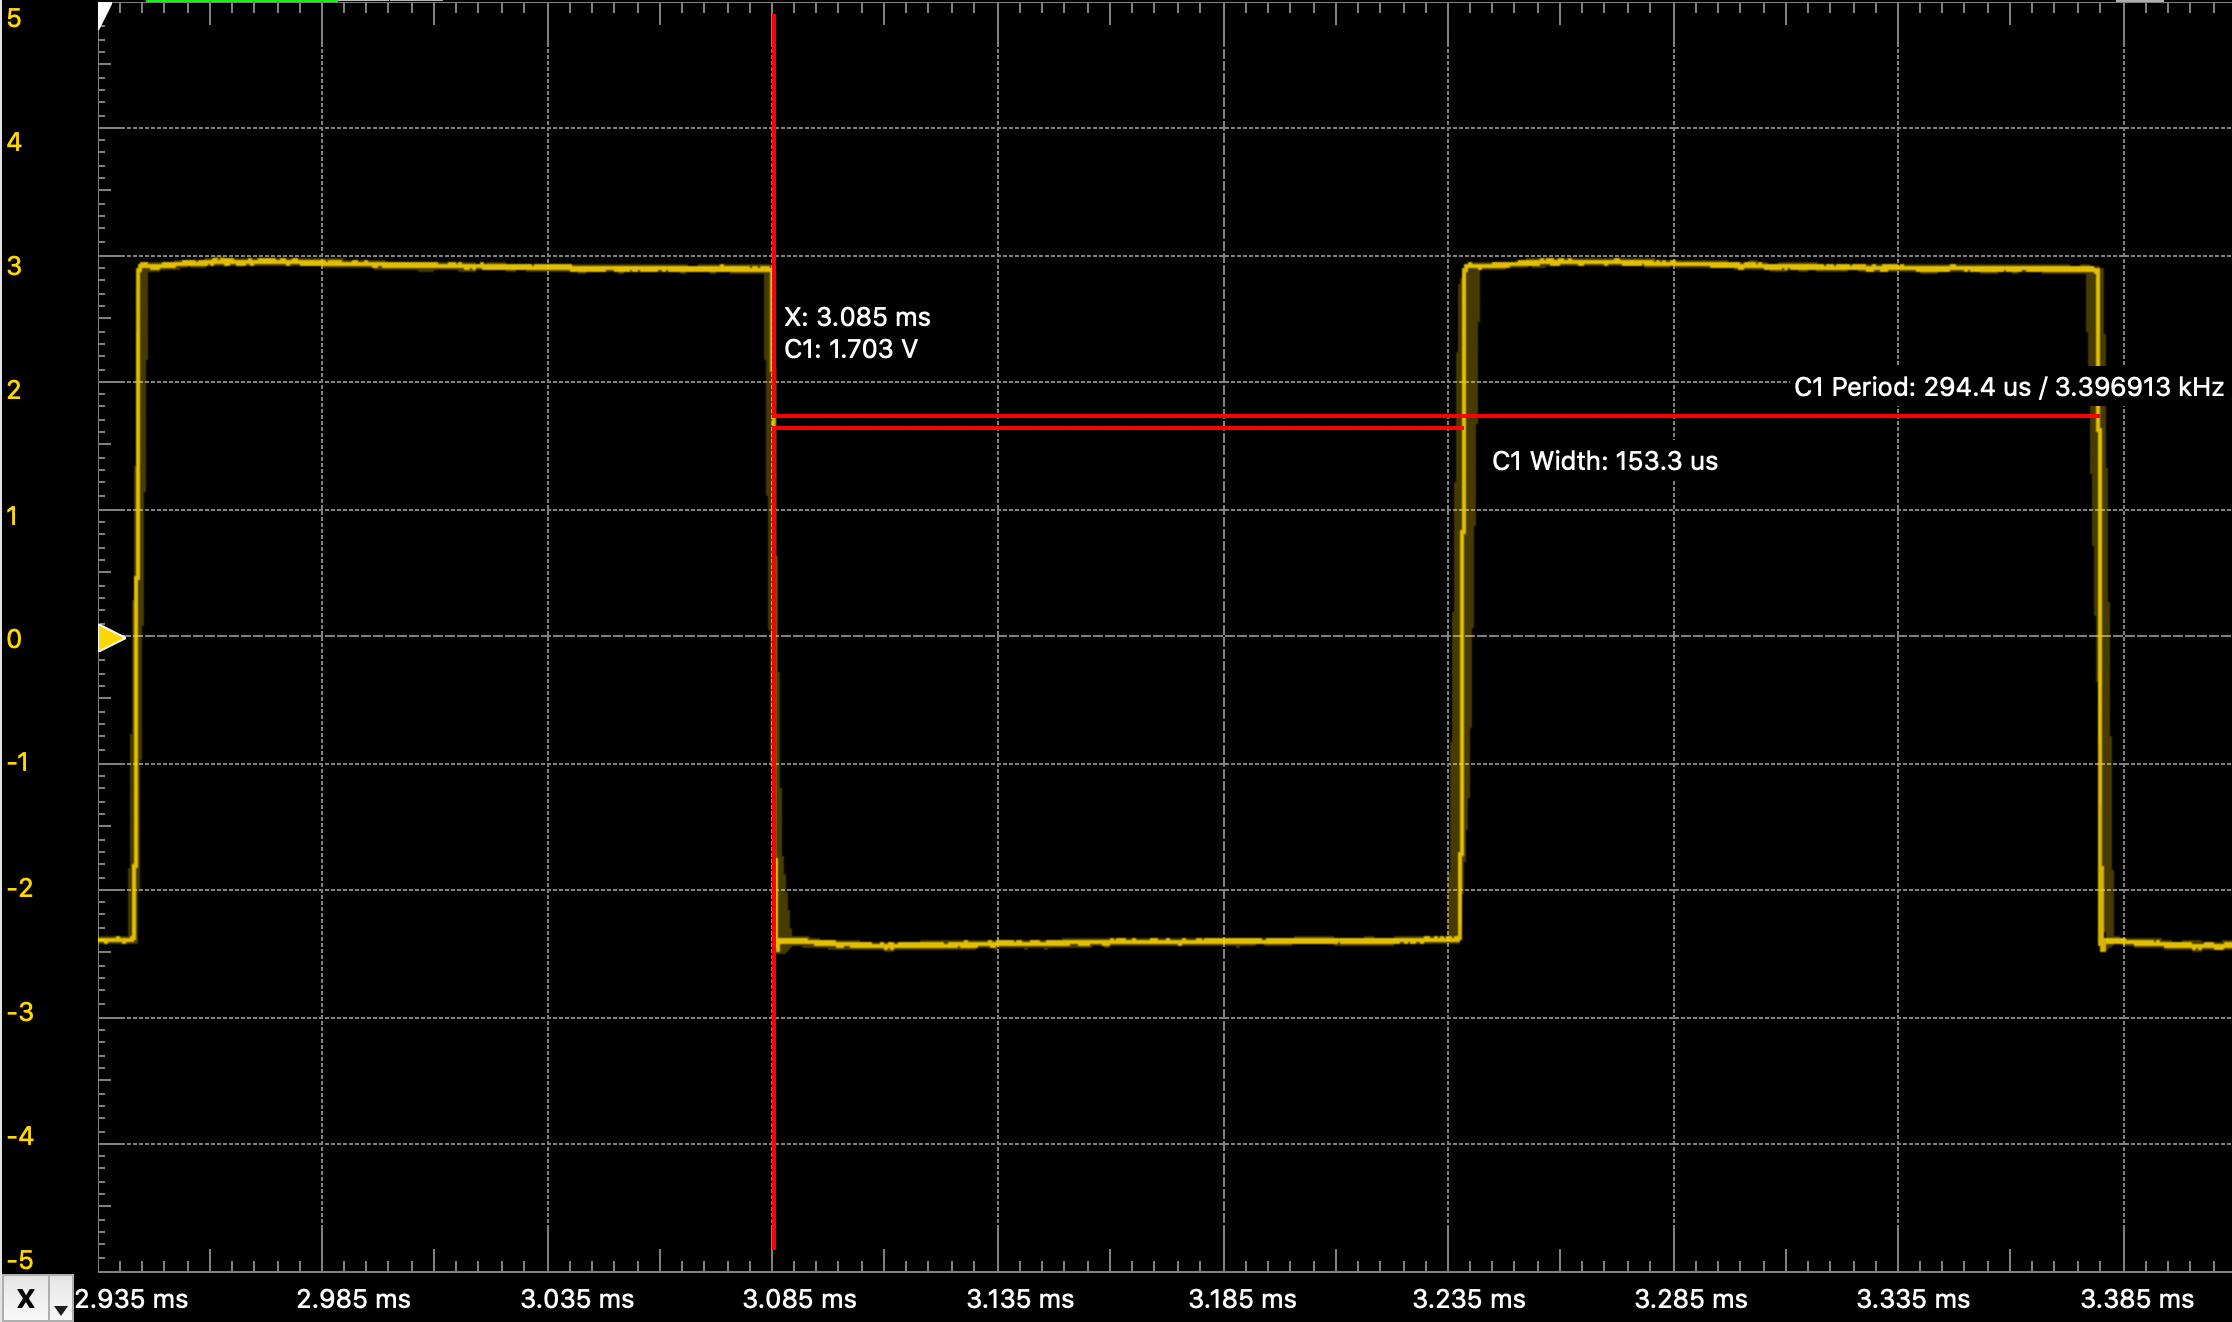
\includegraphics[width=1.0\textwidth]{img/Bøfret_firkantbølge.png}
    \caption{Firkantsignal buffret. Y-akse: Spenning, X-akse: millisekunder.}
    \label{fig:square_after_buffer}
\end{figure}\\

\newpage
\subsection{3. Ordens lavpass filter}
\label{sec:filter_realisering}
Verdiene brukt i filtrene er vist ved tabell~\ref{table:filter}.
\begin{table}[htbp]
\centering
\begin{tabular}{ |c|c|c|c| } 
\hline
\textbf{Navn} & \textbf{Verdi} & \textbf{Beskrivelse} \\
\hline
$R_i$ & $457\Omega$ & $R_i = R_f$ \\ 
\hline
$R_f$ & $457\Omega$ & Likning~\ref{eq:lavpass_filter} $\implies R_f = 455\Omega$  \\
\hline
$C_f$ & $100$nF & Valgri verdi (likning~\ref{eq:lavpass_filter}) \\
\hline
\end{tabular}
\caption{Verdier brukt i lavpass filteret.}
\label{table:filter}
\end{table}
\\
Slik nevnt i seksjon~\ref{sec:filters}, så kobler vi tre aktive lavpass filter etterhverandre, der første filter vises i figur~\ref{fig:first_filter}.
Her ser vi at firkantsignalet vi hadde som inngangsignal begynner å avrunde topp og bunnpunkt, samt at frekvensen er endret litt. Vi har også en liten forstyrrelse i bunnpunktet. Denn forstyrrelsen ser ikke ut til å utvikle seg videre i de neste filterene, så siden første filter ikke er sluttsignalet, så velges det å ikke kommentere ytterlige om dette.
\\\\
Det 2. filteret er vist i figur~\ref{fig:second_filter}.
Signalet ser mer avrundet ut og nærmer seg et sinussignal, men den er enda for spiss i topp og bunnpunktene, så vi velger å filtrere en 3. gang.
\\\\
Det 3. filterert er vist i figur~\ref{fig:third_filter}.
Her er det tydelig noe som likner på et sinussignal.
\\\\
Selv om det ble valgt motstandsverdier som vil gi en forsterkning $A = \frac{R_f}{R_i} = 1$, så har signalet minket i styrke, men fremdeles større enn $A$ fra tabell~\ref{table:slutt_resultat}. \\
Reduksjonen i signalet skjer i RC-kretser når man har et AC signal, som er årsaken til å bruke et aktivt filter, slik at hvis signalet blir for svakt kan man øke $R_f$ for å få et sterkere signal.
\\\\
Fra figurene kan vi også se at signalet har fått en liten negativ offset, som kommer fra op-ampenes funksjonalitet. Verdien på denn offseten er oppgit i databladet for op-ampens modellnr.
\newpage
\begin{figure}[htbp]
    \centering
    \includegraphics[width=1.0\textwidth]{img/Første_filter.png}
    \caption{Første filtrering av firkantsignalet. Y-akse: Spenning, X-akse: millisekunder.}
    \label{fig:first_filter}
\end{figure}\\
\newpage
\begin{figure}[htbp]
    \centering
    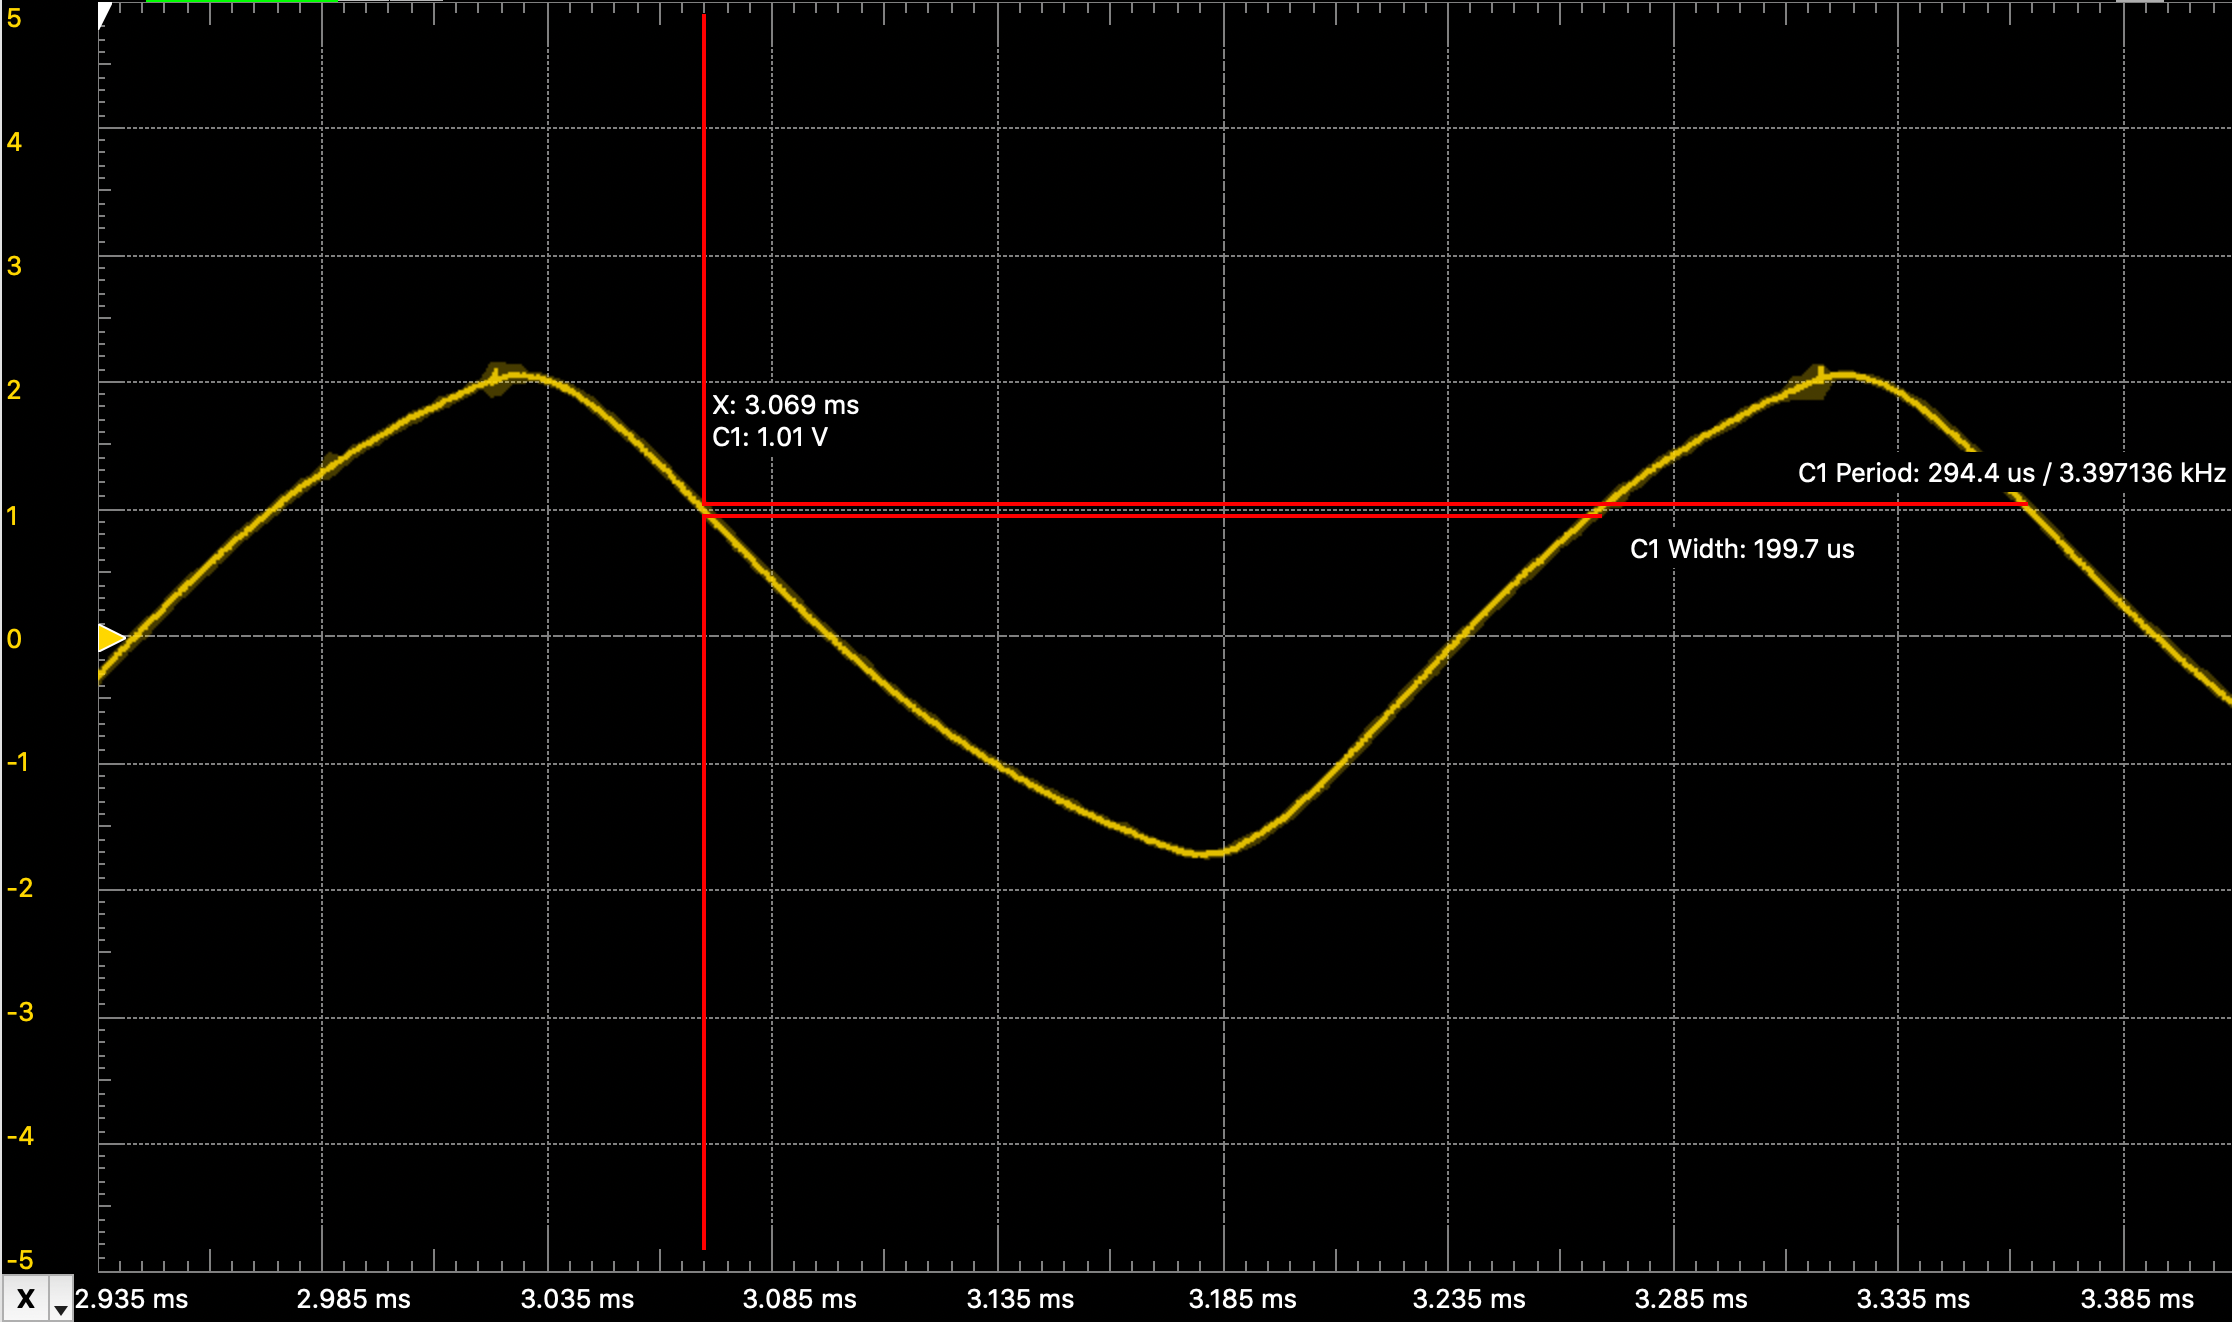
\includegraphics[width=1.0\textwidth]{img/Ande_filter.png}
    \caption{Ande filtrering av firkantsignalet. Y-akse: Spenning, X-akse: millisekunder.}
    \label{fig:second_filter}
\end{figure}\\
\newpage
\begin{figure}[htbp]
    \centering
    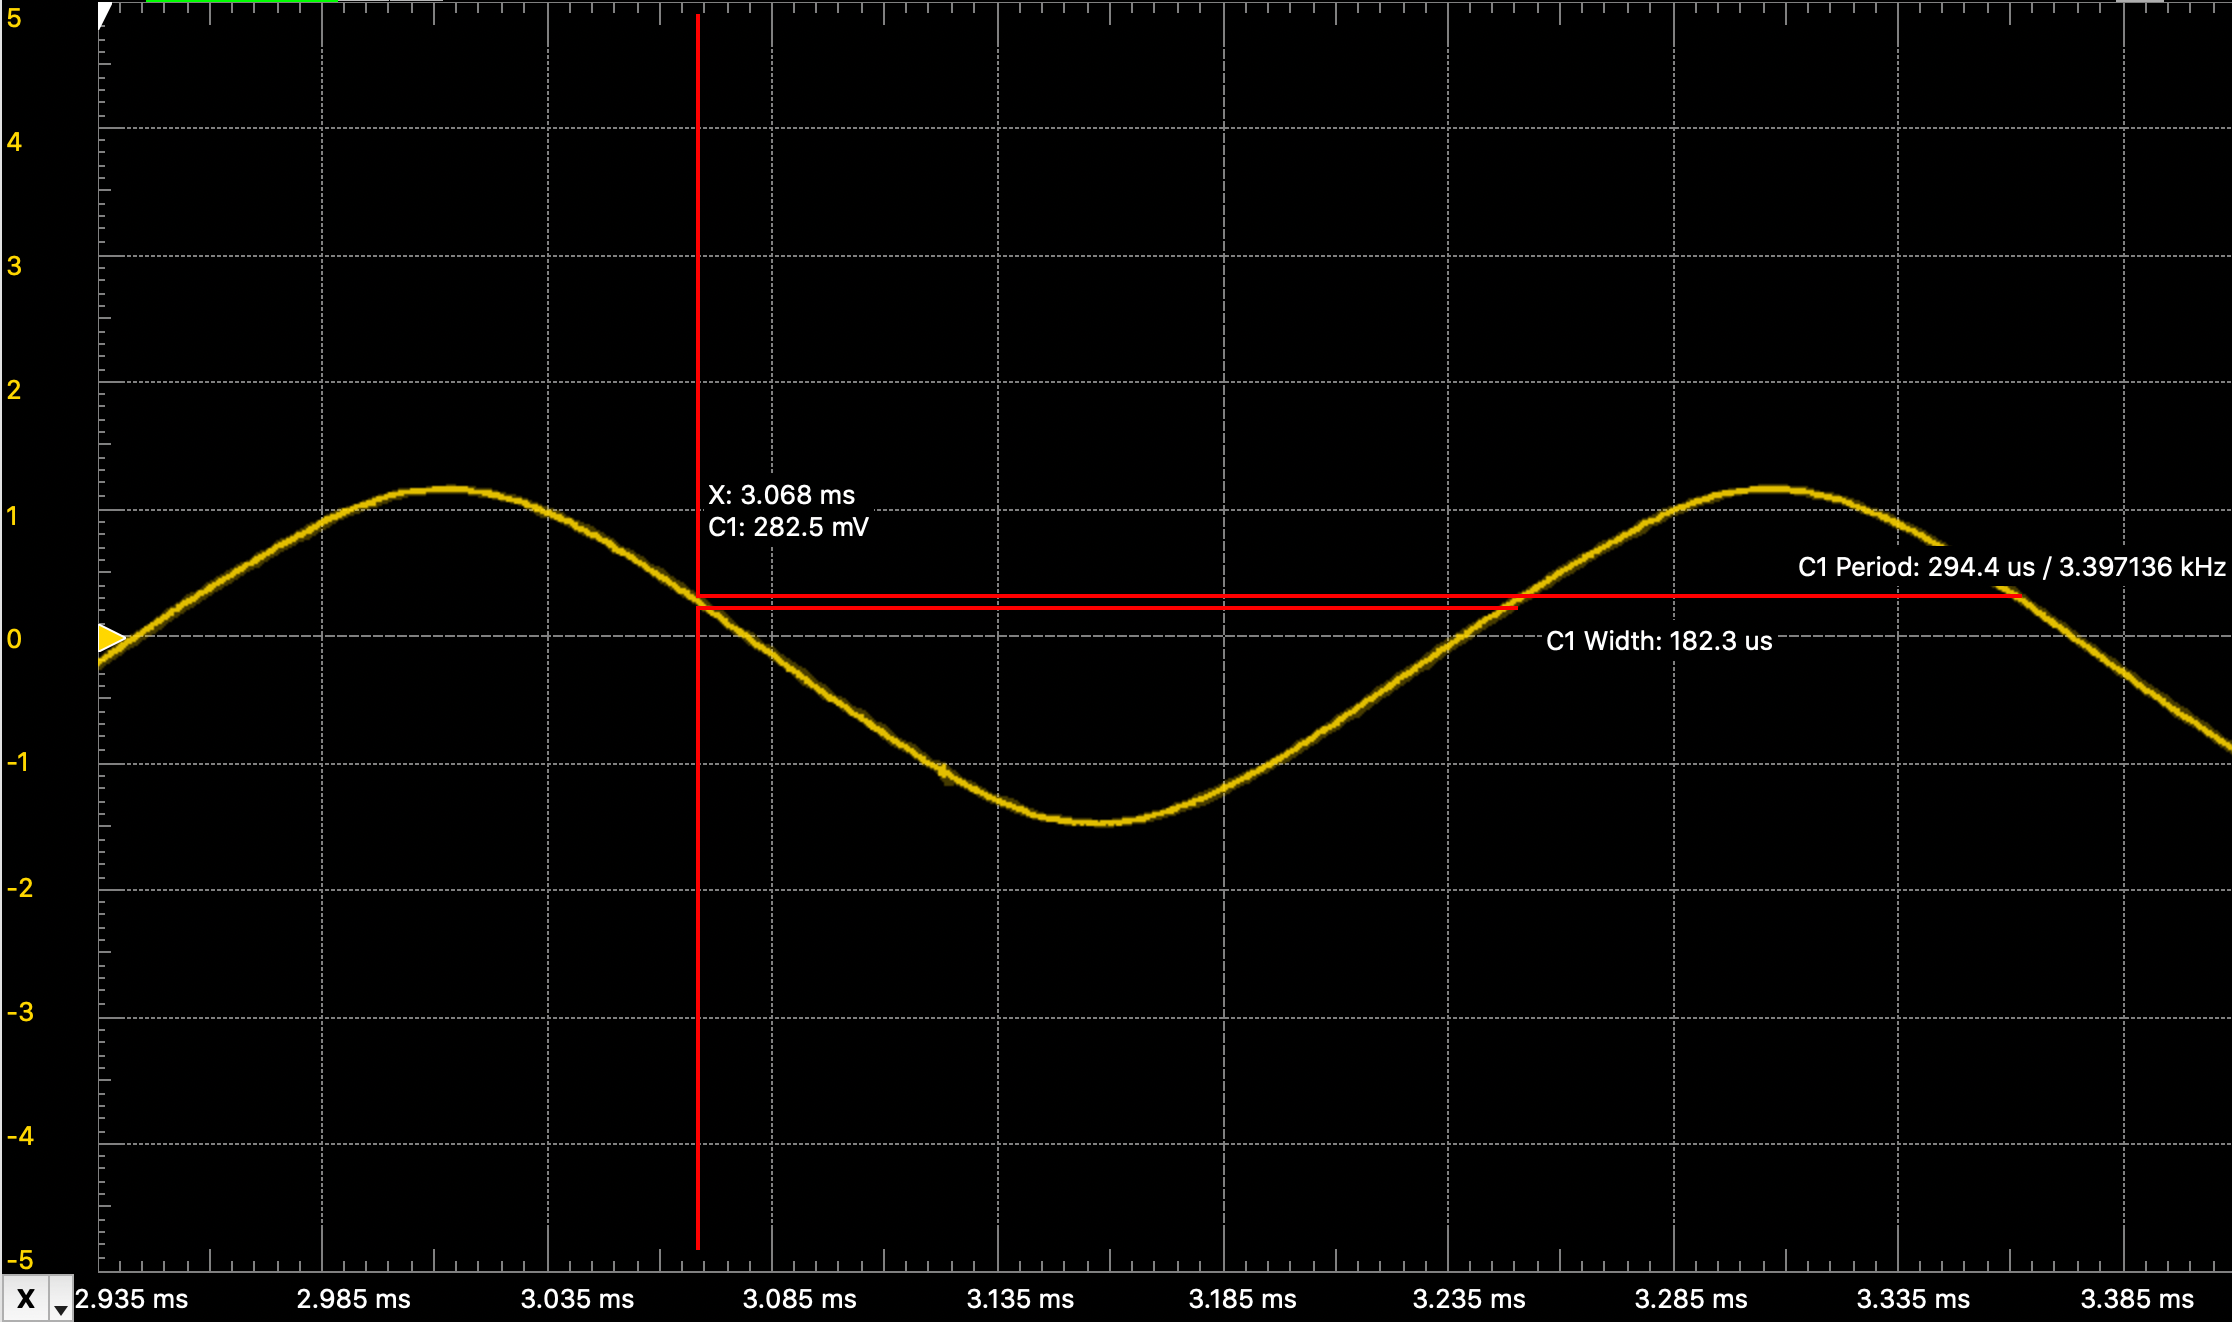
\includegraphics[width=1.0\textwidth]{img/tredje_filter.png}
    \caption{Tredje filtrering av firkantsignalet. Y-akse: Spenning, X-akse: millisekunder.}
    \label{fig:third_filter}
\end{figure}\\

\newpage
\subsection{Nivåregulatoren \& Offset-system}
Verdiene brukt i nivåregulatoren og offset-systemet er vist ved tabell~\ref{table:filter}.
\begin{table}[htbp]
\centering
\begin{tabular}{ |c|c|c|c| } 
\hline
\textbf{Navn} & \textbf{Verdi} & \textbf{Beskrivelse} \\
\hline
$R_{D1}$ & $5000\Omega$ & Likning~\ref{eq:spenningsdemper} \\ 
\hline
$R_{D2}$ & $1000\Omega$ & Valgfri verdi (likning~\ref{eq:spenningsdemper}) \\
\hline
$V_i$ & $5$V & Bruker $V_+$ som spenningskilde. \\
\hline
$R_r$ & $1000\Omega$ & Valgfri verdi (likning~\ref{eq:spenningsdeling_offset}) \\
\hline
$R_{os}$ & $6174$\Omega & Likning~\ref{eq:spenningsdeling_offset} $\implies R_{os} = 6142.9\Omega$ \\
\hline
$V_{os}$ & $0.7$V & $V_{os} = V_0$ \\
\hline
$R_4$ & $1000\Omega$ & Valgfri verdi \\
\hline
$R_A$ & $1000\Omega$ & $R_A = R_B = R_4$ for å unngå forsterkning på $v_6$ \\
\hline
$R_B$ & $1000\Omega$ & Nevnt over. \\
\hline
\end{tabular}
\caption{Verdier brukt i nivåregulatoren og offset-systemet.}
\label{table:offset}
\end{table}
\\
Det endelige signalet $v(t)$ er vist i figur~\ref{fig:end_signal}. Her ser vi at vi har en god tilnærming av riktig offset $V_0$ og en amplitude som er ca. lik $A$ fra \ref{table:slutt_resultat}.
Den endelige frekvensen av $v(t)$ har en endring på 0.7\% fra firkantsignalet $v_2$ sin frekvens. \\
Dersom vi kan endre motstandsverdiene i firkantgeneratoren til å gi riktig frekvens, så vil resten av systemet ha en frekvensnøyaktighet som er innenfor kravet satt i seksjon~\ref{sec:innledning}.
\\\\
Støyet vi kan observere i figur~\ref{fig:end_signal} kan komme fra at signalstyrken er minket såpass mye fra figur~\ref{fig:third_filter}. Støyet forblir stabilt ved endring av amplituden, og vi observerer nå at dette støyet forblir en større del av signalet.
\\\\
Ved bruk av en spektrumanalysator på et frekvensområde $<0$Hz$, \:40$kHz$>$, så vises 5 harmoniske frekvenser.
Det er mulig å finne SDR ved å bruke spektrumanalysator eller ved å regne ut RMS verdien til fundamentalfrekvensen $V_x$, samt summen av de andre harmoniske signalene $V_\hat{x}$:
\begin{equation}
    \textit{SNR} = 10 \log \left( \frac{V^2_x}{V^2_\hat{x}} - V^2_x \right).
\end{equation}
\\
Sprektrumsanalysatoren gir en SDR$\in<25.6$dB$, 29.5$dB$>$. Støyet endrer seg med tiden, som gjør at vi ikke får en stabil måling. Dette signalet er godt nok, ifølge kravet som ble satt i seksjon~\ref{sec:innledning}.
\newpage
\begin{figure}[htbp]
    \centering
    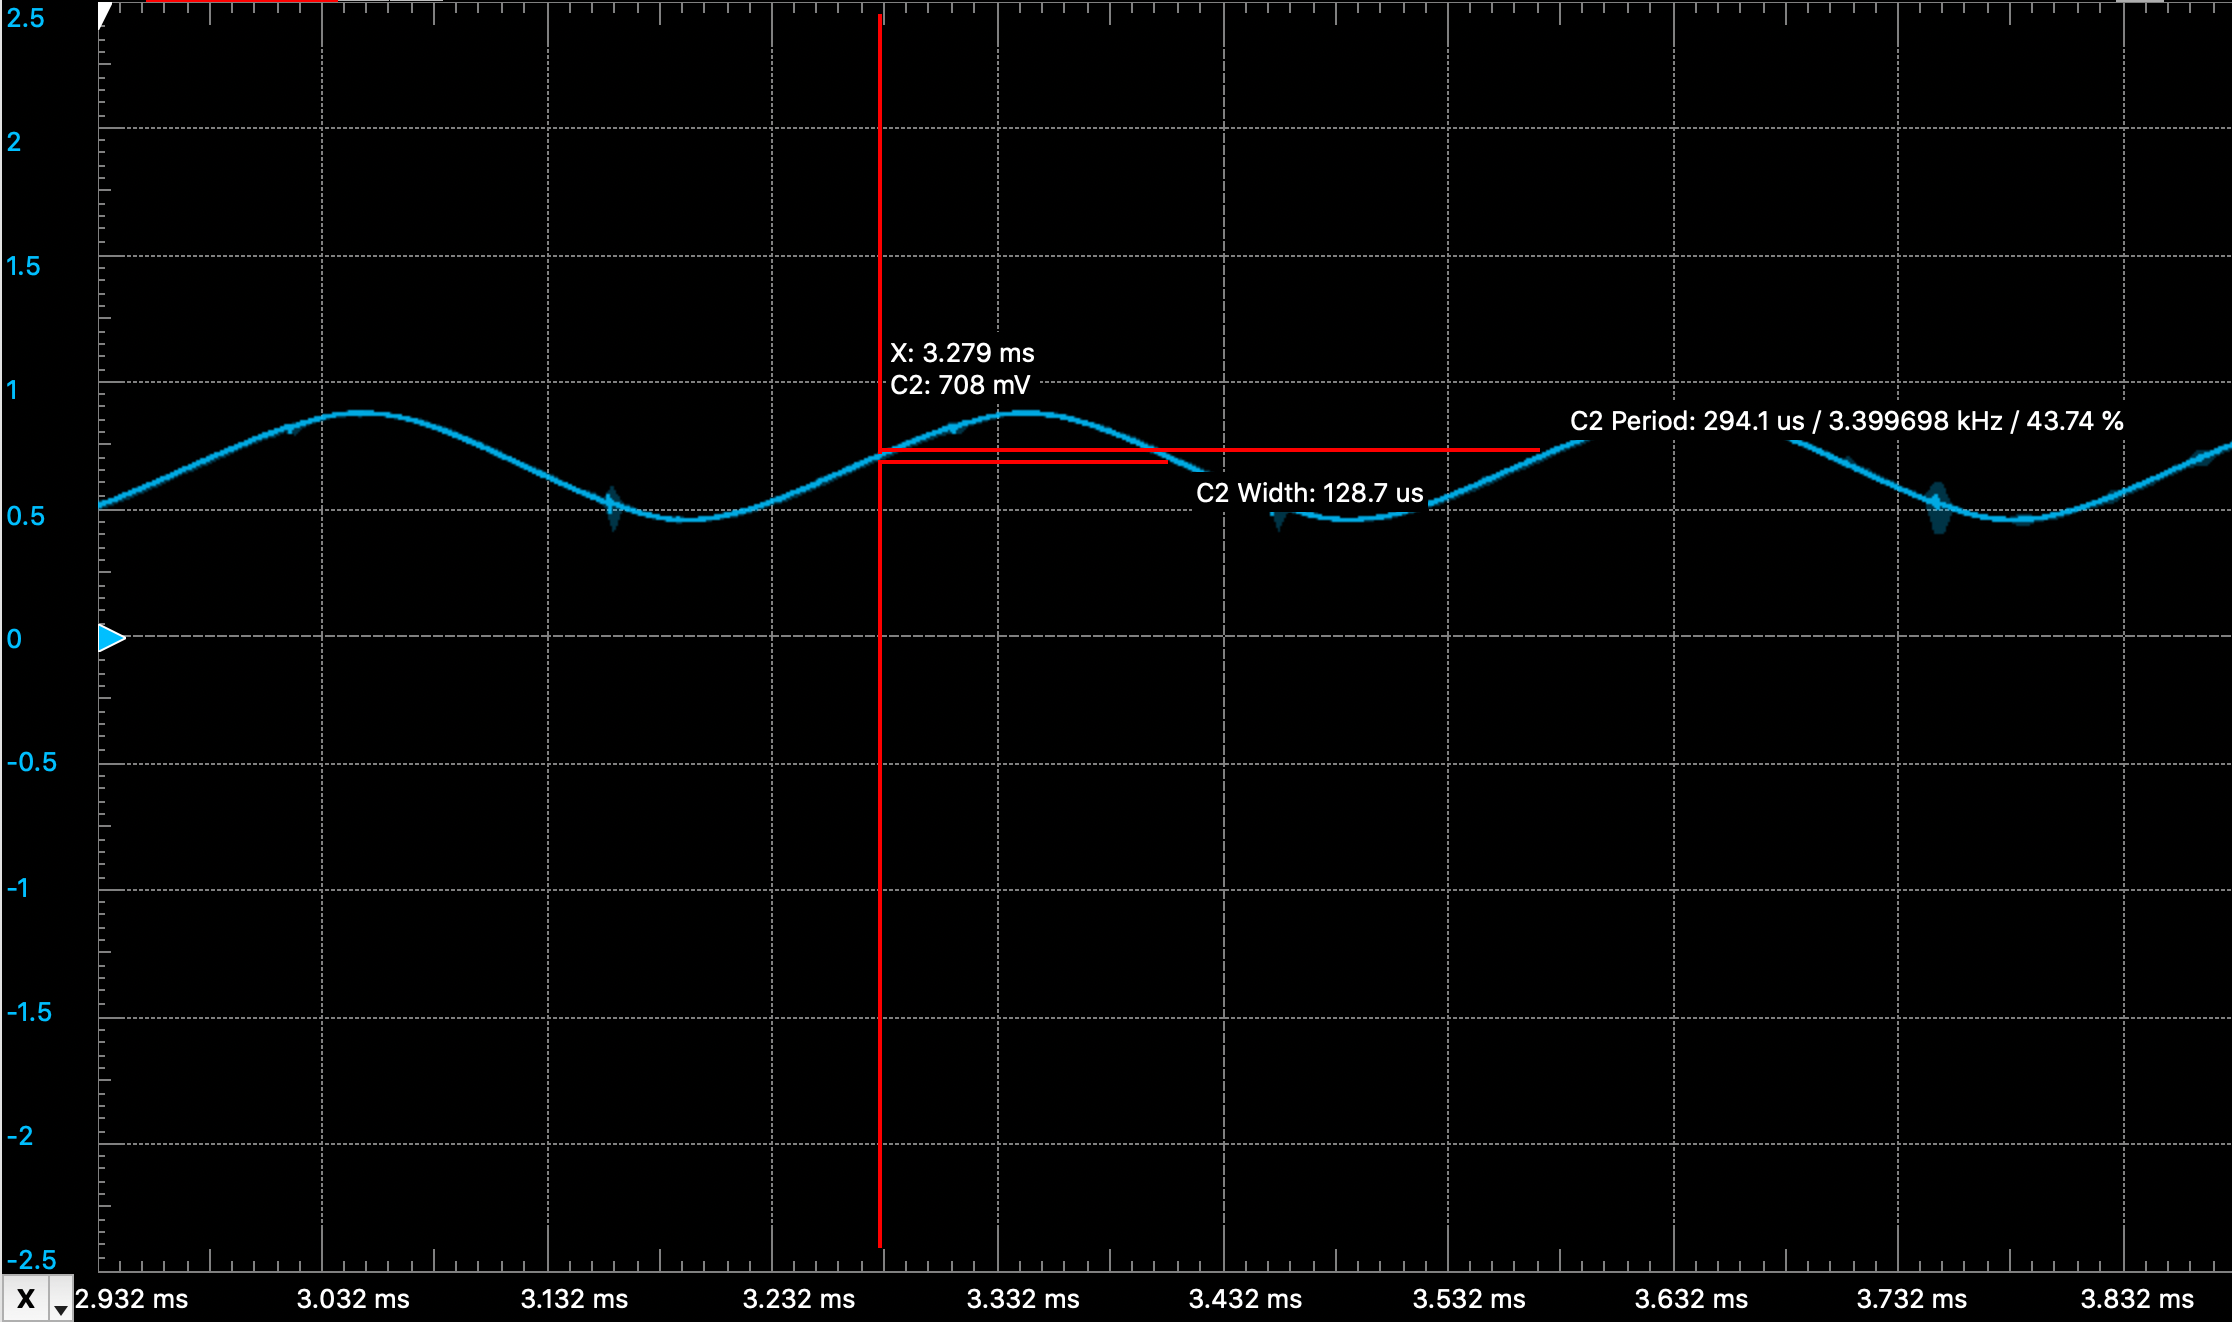
\includegraphics[width=1.0\textwidth]{img/ferdig signal.png}
    \caption{Sinussignalet $v(t)$ med offset og ønsket størrelse. Y-akse: Spenning, X-akse: millisekunder.}
    \label{fig:end_signal}
\end{figure}\\
\newpage
\begin{figure}[htbp]
    \centering
    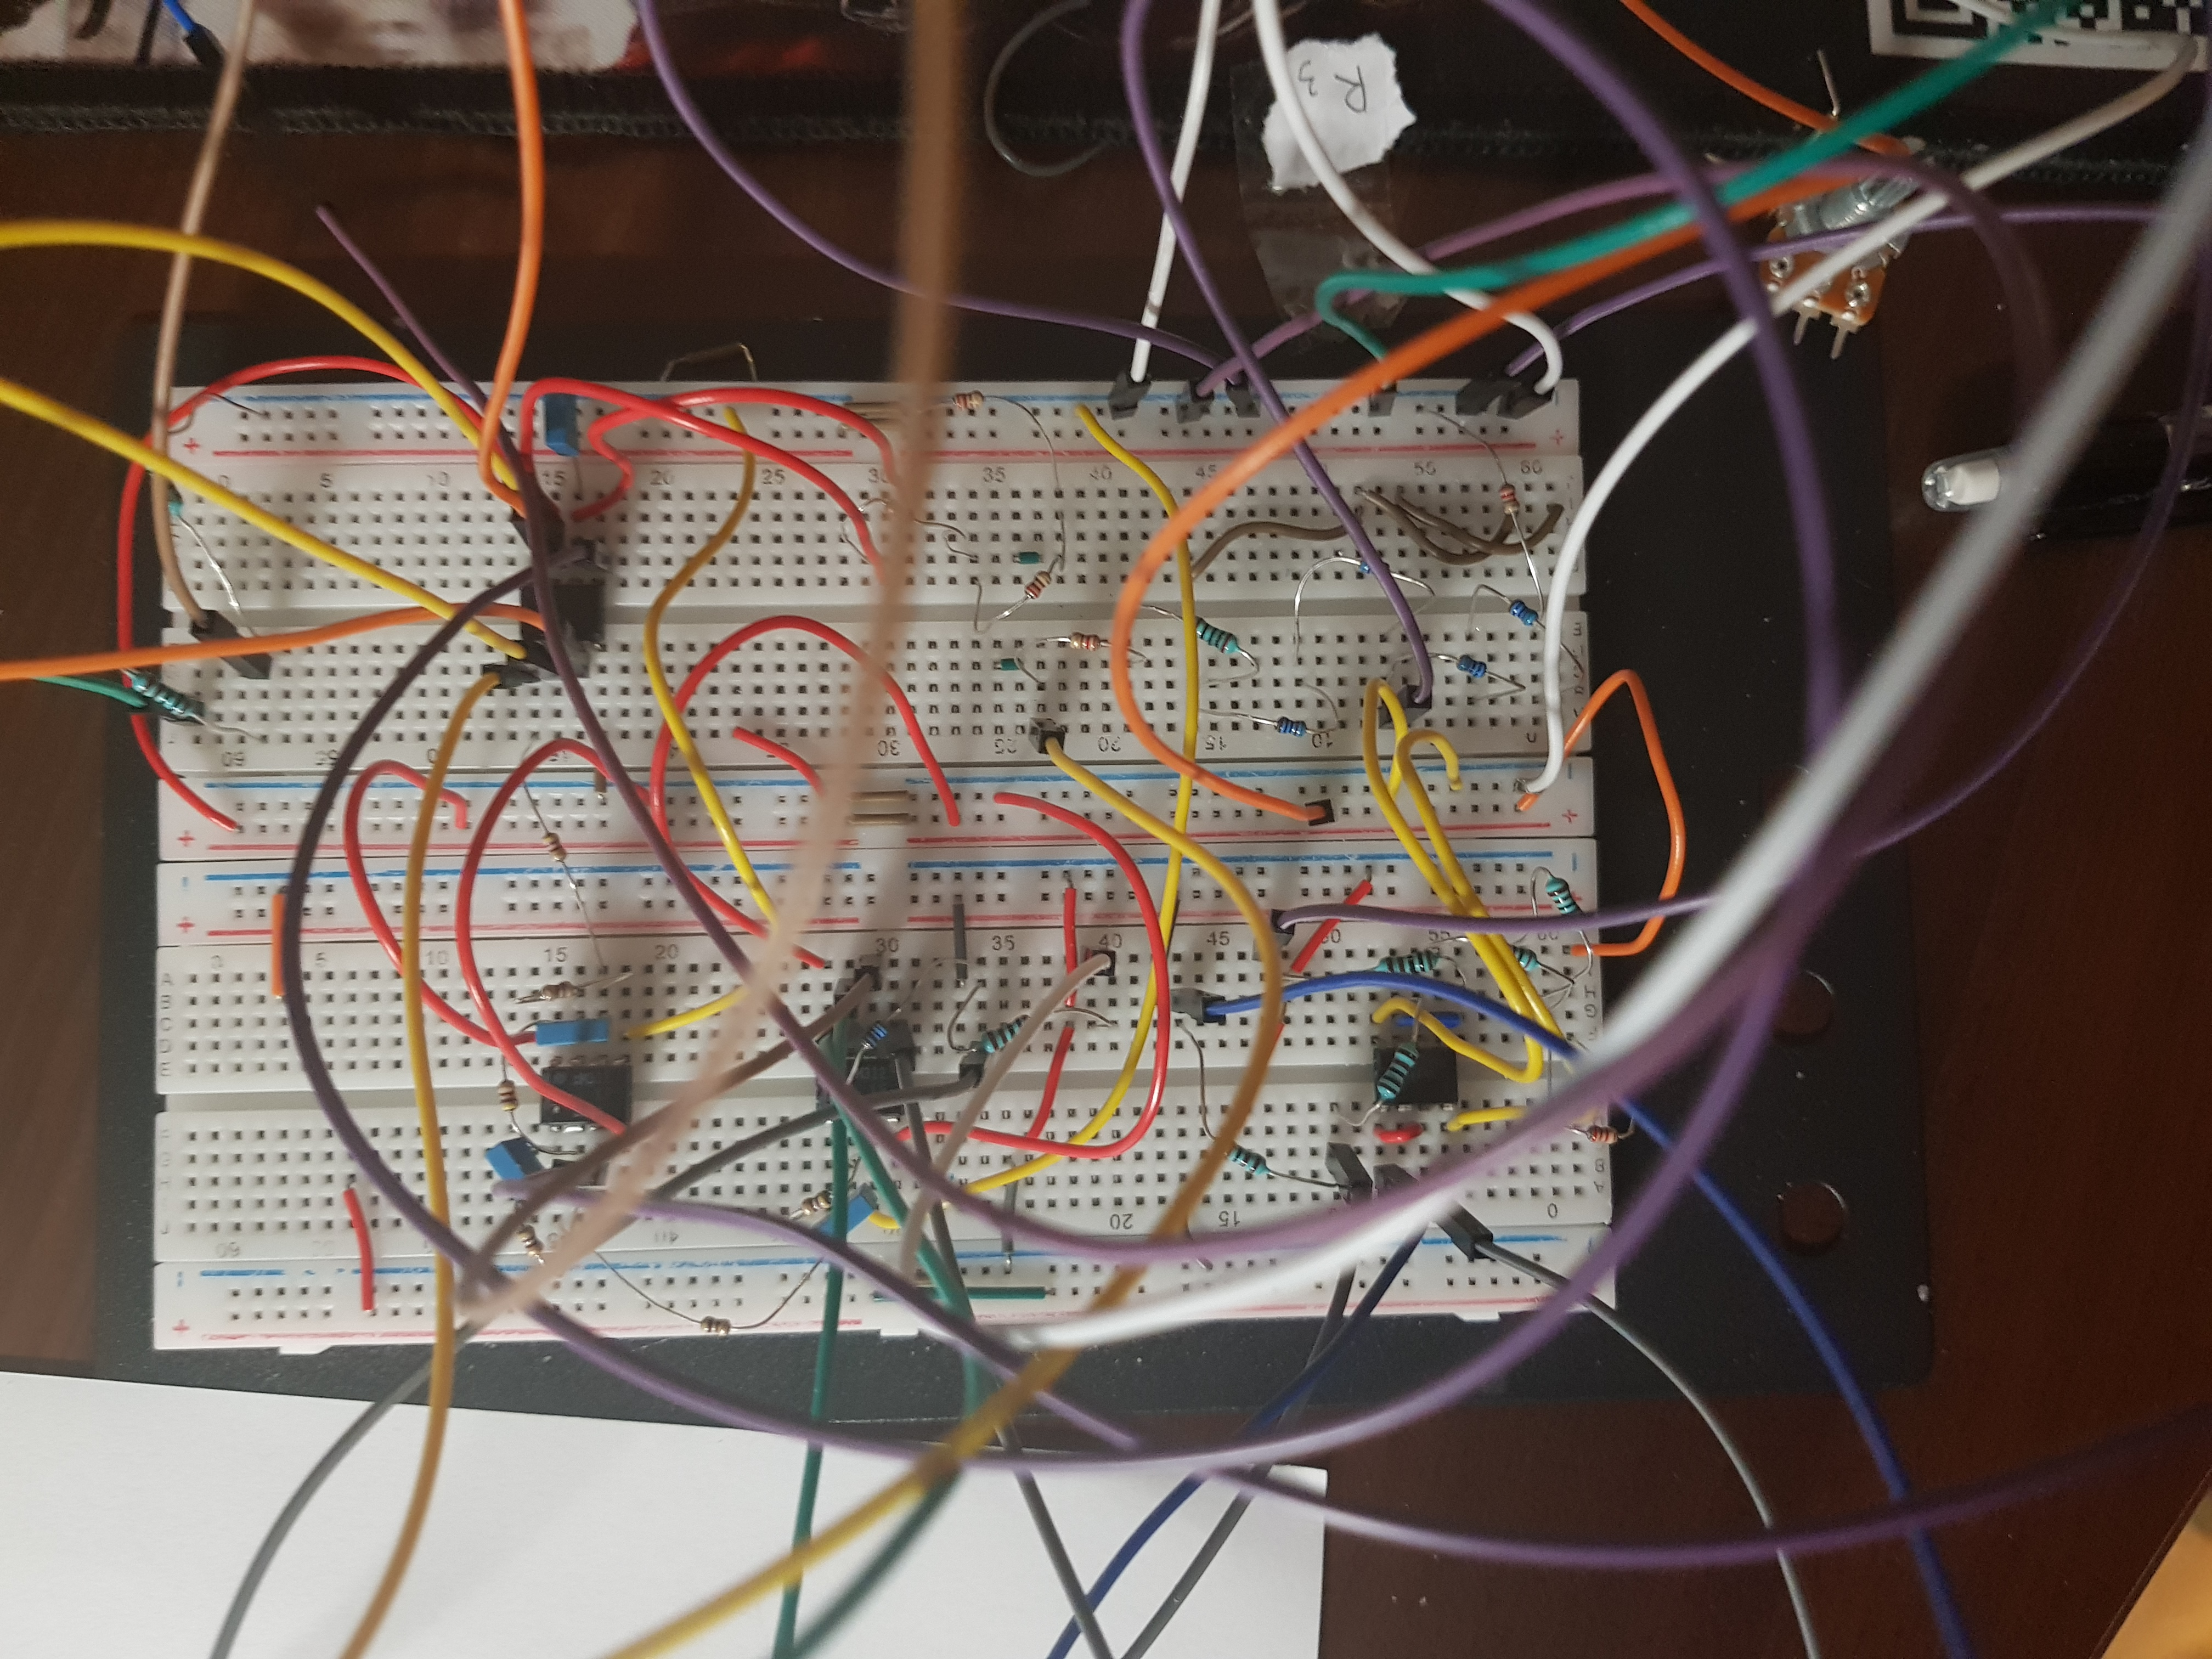
\includegraphics[width=1.0\textwidth]{img/20210606_001211.jpg}
    \caption{Realisert krets.}
    \label{fig:real_krets}
\end{figure}\\
\newpage

\section{Konklusjon}
\label{sec:konklusjon}
Sinusgeneratoren gir et godt tilnærmet sinusignal. Med en akseptabel støymengde, som er testet opp til 40kHz.
For en bedre SDR, så kan f. eks kortere kabler brukes i den realiserte kretsen vist ved figur~\ref{fig:real_krets}.
Frekvensen beholdes godt nok gjennom kretsen. Det eneste er at motstandsverdiene for firkantgeneratoren må endres, ved eventuelt et potensiometer. 

%Bibliografi: Legg til flere elementer ved å legge til flere \bibitem:--------
\phantomsection
\addcontentsline{toc}{section}{Referanser}
\begin{thebibliography}{99}

\bibitem{r1} Non-Inverting Operational Amplifier, 2021, Electronics-tutorials, \\
\href{https://www.electronics-tutorials.ws/opamp/opamp\_3.html}{https://www.electronics-tutorials.ws/opamp/opamp\_3.html}
\bibitem{r2} Square Wave Generator, 2021, Elprocus, \\
\href{https://www.elprocus.com/what-is-a-square-wave-generator-circuit-diagram/}{https://www.elprocus.com/what-is-a-square-wave-generator-circuit-diagram/}

\bibitem{r3} Active Low Pass Filter, 2021, Electronics-tutorials, \\
\href{https://www.electronics-tutorials.ws/filter/filter\_5.html}{https://www.electronics-tutorials.ws/filter/filter\_5.html}

\end{thebibliography}


\end{document}